% !TeX root = ../main.tex

\chapter{相关工作}

\section{着色器程序优化}

\subsection{着色器程序语言}

作为一类领域专用语言 (DSL, Domain Specific Language),着色器程序语言是应用在图形 API 中,负责增强和替换图形管线中相应部分固定功能的程序和程序片段编写所用的程序设计语言。

% SEE https://www.nvidia.com/docs/IO/8227/GDC2003_OGL_ARBVertexProgram.pdf and https://www.nvidia.com/docs/IO/8228/GDC2003_OGL_ARBFragmentProgram.pdf

图形程序语言经历了一个从简单到复杂、从低级到高级的过程,这种转变趋势可以从不同的图形 API 中得到证明。2002 年,OpenGL 1.4 引入了 ARB 扩展 ARB\_vertex\_program,其中使用了较为低级的汇编指令形式来描述顶点变换阶段的用户自定义功能。在之后一年的 OpenGL 1.5 中,OpenGL 着色器程序语言 (GLSL, OpenGL Shading Language) 1.0 版本被引入到 ARB 扩展 ARB\_vertex\_shader 和 ARB\_fragment\_shader 中,并在之后发展迭代,和 OpenGL 标准本身一起演进。

在由 Microsoft 公司主导的 DirectX 图形 API 中,也有类似的发展轨迹。2000 年的 Direct3D 8.0 中,Microsoft 公司引入了使用平台无关的汇编指令来描述顶点变换和像素着色阶段功能的着色器程序模型。之后,在 2002 年的 Direct3D 9.0 中,Microsoft 公司进一步设计了使用高级语言形式来描述顶点变换和像素着色阶段功能的高层次着色语言 HLSL (High Level Shading Language),并且在随后的标准演进中不断增加新功能。

然而,GLSL 和 HLSL 等高层次着色器程序语言因其较为丰富的语法特性,其处理和向 GPU 底层指令的转换均较为复杂。针对这类问题,Khronos Group 提出了一种统一的图形和计算中间表示 (IR),并将其命名为 SPIR-V。经过多年的投入,SPIR-V 成为了 Vulkan 图形 API 的着色器程序输入格式,并且围绕 SPIR-V 有丰富的编译器设施。

本文所构造的预测器即基于 SPIR-V 中间表示。这样的技术选型有如下两方面的优点:首先,SPIR-V 拥有成熟的转译器 (transpiler) 生态,GLSL、HLSL 和新型的着色器程序语言 Slang 等均拥有向 SPIR-V 进行转译的工具;其次,SPIR-V 技术设计上即方便进行编译器的编写和编译变换,其采用线性 IR 表示,并有简洁清晰的语言规范,成熟可靠的语言优化器等,对本文所述的指令统计阶段所需要的指令编排工作有一定的帮助。

\subsection{着色器程序优化和简化}

图形 API 本身为了兼容各种不同厂商和架构的底层 GPU 硬件实现,其所希望用户程序本身呈递的着色器程序是贴近高级语言语义的、基本未经历过设备相关的优化、也没有附加很多设备相关语义的着色器程序源语言文本或中间表示。然而,出于图形程序的性能考虑,图形程序员和 GPU 设备厂商通常希望对着色器程序进行一定意义上的优化,使得其在不同或特定平台能拥有较好的实时性能。这样的要求催生了对着色器程序优化和简化的相关工作的探索。

GPU 设备厂商应用的着色器程序优化主要发生在图形程序启动时。此时,图形程序会经由图形 API 向设备驱动呈递着色器程序源码或其中间表示,此时设备驱动中的图形流水线编译器模块将会像传统的 CPU 程序编译器一样,进行源码的中间表示生成,以及编译器后端的设备无关优化、设备相关优化、寄存器分配和指令生成。在这个过程中,编译的速度和编译生成的指令序列的质量都是编译器追求的目标。即便如此,\cite{8366956} 仍然发现设备厂商的驱动并没有充分利用各种可能的着色器程序离线优化机会。\cite{8891638} 也发现,对于输入比较确定的着色器程序,仍然存在进一步优化的空间。

设备驱动中的优化需要基本保证优化后的程序符合原来输入程序的运行结果,但是对于图形应用来说,进行输出完全符合原状的着色器程序优化对于如游戏等应用场景来说并不是必需的。故而,有一系列工作 \cite{10.1145/3528233.3530722, 10.1145/2661229.2661276, 10.1145/2070781.2024186, 10.1145/2816795.2818104, 9815871} 探索了如何在有损条件下,权衡画面表现和运行性能来进行着色器程序简化。这些工作通常使用遗传算法 (GP, Genetic Programming) 和贪心算法来实现。在遗传算法的每步迭代中,这些工作通常会考虑各种可能对画面造成损失的简化方法:例如,将决定着色器输出的表达式的某个子表达式的值替换为零或该表达式在各种光照条件下的求解结果的平均值,或者将片段着色器阶段进行计算的值移动到顶点着色阶段等。为了进一步加快遗传算法的变异-迭代过程,\citet{10.1145/3528233.3530722} 提出了ShaderTransformer,该方法利用深度学习提出了一个着色器简化变体的渲染质量质量预测器。

值得注意的是,目前在有损着色器简化的工作通常局限于使用比较简单的启发式算法来表示着色器的运行时开销\cite{10.1145/2816795.2818104, 10.1111/cgf.13482, 10.1145/3528233.3530722},又或者每次评估变异后的着色器程序时进行单独的测量运行\cite{10.1145/2661229.2661276}。我们有理由相信,本文提出的预测器将可以在不需要在目标平台上进行单独执行的条件下,对变异后着色器的运行时间开销做出更精确的预测。

\section{程序语言理解}

\subsection{语言模型}

语言模型是自然语言或程序语言的概率模型。一个语言模型通常定义了语言中文本 $\{l_1, l_2, ..., l_m\}$ 与分词后形成的词元 $\{w_1, ..., w_n\}$ 的对应关系,以及对于句子 $ w_1, ..., w_{i-1} $ 来说,词元 $ w_i$ 出现几率的概率模型 $P(w_i|w_{i-1}, ..., w_{1})
$。

% TODO: add bigram, trigram, ...

对于语言模型来说,将源语言文本转换为词元的分词过程对后续处理有一定影响。对于自然语言文本,各个单词出现的机率并不是均匀的,而对于出现次数过于稀疏的生僻词语,语言模型对其的概率估计总体来说较为困难。为了解决这个问题,BPE (Byte-Pair Encoding) \cite{sennrich-etal-2016-neural} 使用了一种被称为 subword 的单位来进行分词,并被 SentencePiece \cite{kudo-richardson-2018-sentencepiece} 等方法使用。

\subsection{注意力机制与 Transformer 网络}

注意力机制是模仿认知活动中注意力活动的一类神经网络机制。在使用注意力机制的网络中,通常会根据序列内容,为序列中的每个词元生成一个软的权重,并根据部分或全部序列中词元的权重来进行后续的计算。

基于 \citet{bahdanau2016neural} 中注意力机制的工作,Google 公司在 2017 年提出了被称为 Transformer \cite{Vaswani2017AttentionIA} 的神经网络结构,在自然语言处理的各类任务上均取得了巨大的成功。Transformer 网络总的结构如图 \ref{fig:transformer_overview} 所示。

\begin{figure}[h]
  \centering
  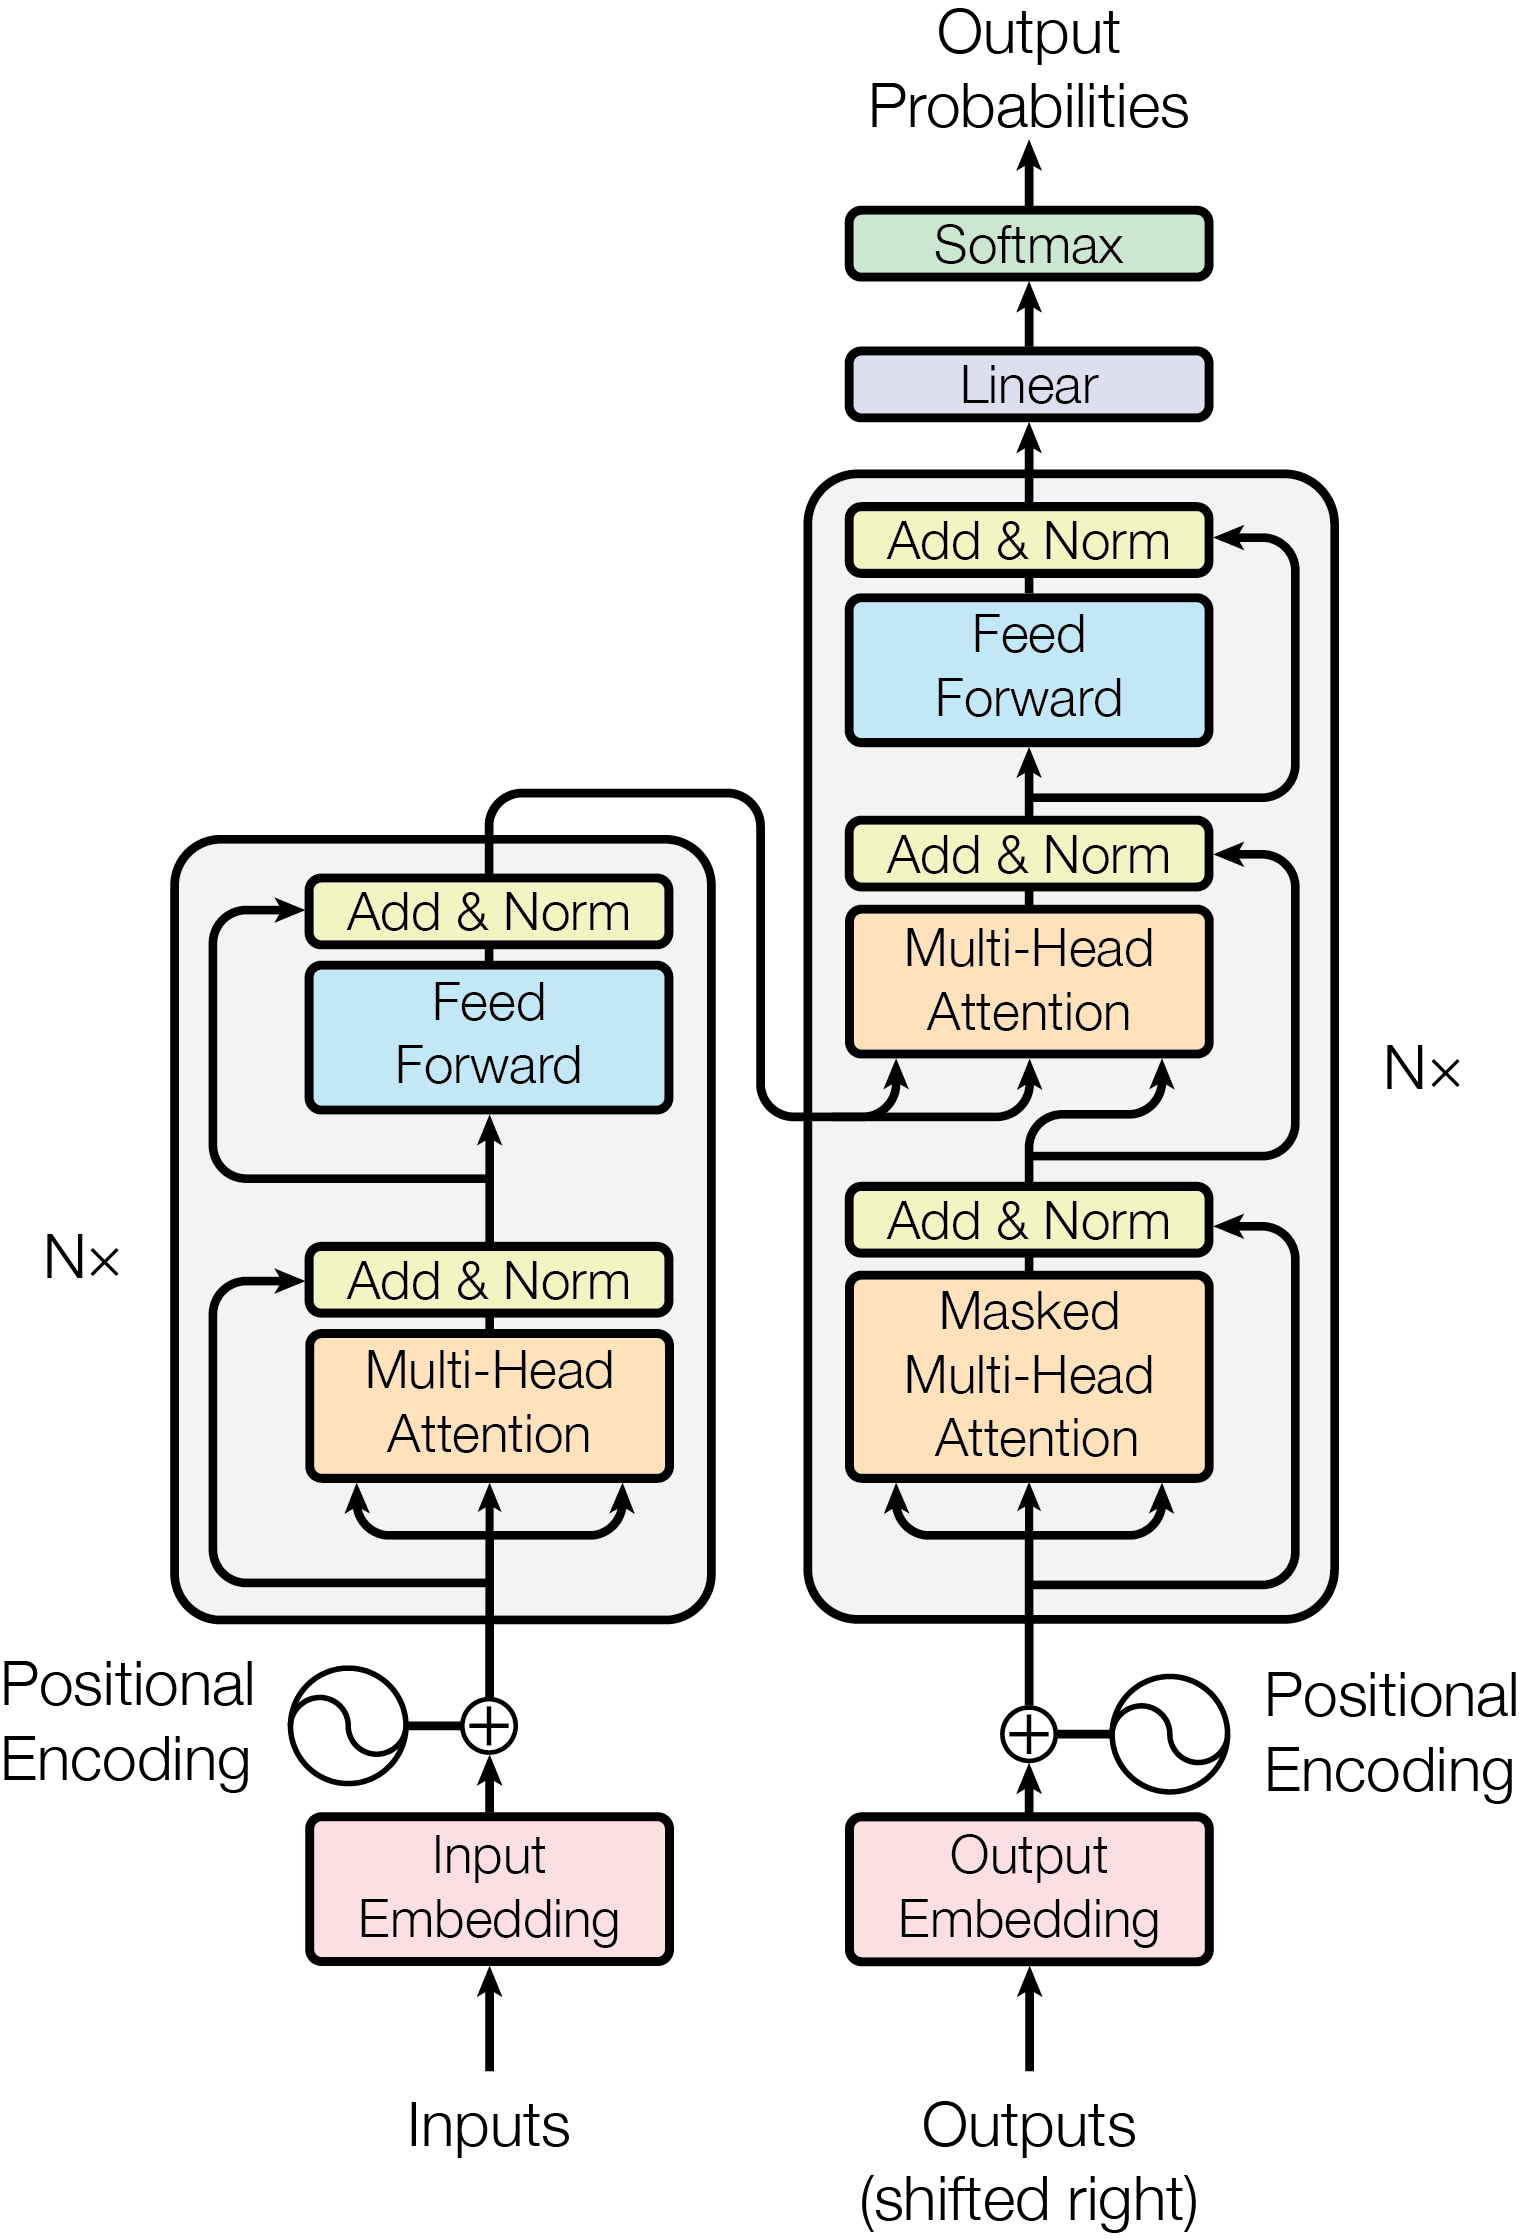
\includegraphics[width=0.5\linewidth]{figures/Transformer-Arch.png}
  \caption{Transformer 网络结构总览 (图片来源 \citet{Vaswani2017AttentionIA})}
  % \Description{}
  \label{fig:transformer_overview}
\end{figure}

% generated by gpt3.5; TODO: rewrite

原始版本的 Transformer 模型的网络结构主要由编码器 (Encoder) 和解码器 (Decoder) 两个组件构成。Tranformer 的编码器负责将输入的序列转换为相应长度的特征向量,而 Transformer 的解码器则会利用这些特征向量来生成输出序列。

Transformer 的编码器和解码器都由多个相同的基本层堆叠而成,其每个基本层都由两个子层组成:多头自注意力层 (Multi-Head Self Attention) 和前馈神经网络层 (Feed-Forward Neural Network)。这两个子层之间使用层归一化 (Layer Normalization) 和残差连接 (Residual Connection) 来连接在一起;同时,在层内的一些位置还会加入 Dropout 层进行归一化。

多头自注意力层由多个相同结构的自注意力层构成。在每个自注意力层中,输入的序列会被分别线性变换到三个被称为查询 (Query)、键 (Key) 和值 (Value) 的序列。随后,这三个序列会进行一个被称为缩放点积注意力 (Scaled dot product attention) 的操作
$$
\operatorname{Attention}(Q, K, V) = \operatorname{softmax}\left(\frac{Q K^T}{\sqrt{d_k}}\right)V,
$$
其中 $Q$ 为查询,$K$ 为键,$V$ 为值,$d_k$ 为键的维度。

这种类型的注意力机制可以允许序列中任意的两个位置的词元交换信息,且通过注意力分数来表征了每个位置对其他位置的“重要性”,从而实现了序列中不同位置之间的交互和信息传递。

将维数为词元嵌入维度 $ d_{model} $ 的序列并行的进行多组自注意力操作可以改善模型表现。多个这样的注意力机制进行拼接的结果为多头注意力,其计算方式如下:
$$
\operatorname{MultiHead}(Q, K, V) = \operatorname{Concat}(head_1, ..., head_h) W^{O}
$$
其中 $head_i$ 为第 $ i $ 组独立的进行自注意力计算的计算结果。

多头自注意力层之后,连接的另一个重要模块是前馈神经网络层。该层由两个全连接层组成,并通过 ReLU 函数进行激活,其计算方式如下:
$$
\operatorname{FFN}(x)= \max(0, x W_1 + b_1) W_2 + b_2
$$

原始的 Transformer 中同时使用了编码器和解码器,而编码器和解码器之间还有一个重要的结构:编码器-解码器注意力层 (Encoder-Decoder Attention)。在解码器中,每个位置的输出依赖于编码器中所有位置的输入。为了实现这种全局的依赖关系,解码器的多头注意力层中使用了编码器的输出来作为查询 $Q$ 和键 $K$。

总体来看,Transformer 模型通过自注意力机制和多头注意力机制,有效地捕捉了输入序列中的全局依赖关系,并在许多自然语言处理任务中取得了显著的性能提升。譬如,BERT \cite{devlin-etal-2019-bert} 模型就利用预训练的范式,在 Transformer 编码器的基础上利用掩码语言建模 (Masked Language Modeling) 和后续语句预测 (Next Sentence Prediction) 任务在大规模预料上进行预训练,其在下游任务上只需接受较少的微调即可达到较好的性能。

由于本文提出的预测器需要将整个着色器程序的 SPIR-V 作为模型的输入,这样一来,模型可以接受的序列长度将直接影响其训练和使用时的泛用性。针对于 Transformer 训练时内存占用较高的问题,本文之后提出的预测器中,其骨干部分同时利用了低内存占用的 Memory Efficient Attention \cite{rabe2022selfattention} 注意力实现。

\subsection{程序设计语言理解任务}

程序设计语言可以被看作一种特殊形式的语言,故而很多自然语言处理领域的方法也适用于程序设计语言的相关任务中。在如 Transformer\cite{Vaswani2017AttentionIA} 和 BERT\cite{devlin-etal-2019-bert} 等模型的影响下,业界涌现出了一批用于程序设计语言任务的模型,如 CodeBERT\cite{feng-etal-2020-codebert},GraphCodeBERT\cite{DBLP:conf/iclr/GuoRLFT0ZDSFTDC21} 等。类似的,我们的工作也采用 Transformer 来捕捉着色器指令间的上下文相关性。

根据 \citet{ijcai2022p775} 等人的综述,程序语言理解模型的典型应用包括抄袭检测,代码分类,代码缺陷检测,代码检索等。同时,也存在被设计为捕捉性能相关的语义的一类任务,譬如在 \citet{8091247} 中引入,并被后续工作 \cite{pmlr-v139-peng21b, pmlr-v139-cummins21a} 用于评价模型质量的 OpenCL 异构架构映射任务。该类任务的输入是一系列 OpenCL 核函数 (kernel function),程序语言理解模型需要给出某个具体的核函数在何种平台上运行较快的分类值。我们希望,通过本文的研究过程中收集的着色器性能数据,可以启发出更多关于程序语言模型中进行性能语义理解任务的工作。

\section{程序性能建模}

程序性能建模对于计算机软件架构设计和实现中的众多决策都有比较重大的意义,所以学术界开展了大量的、不同计算平台上的,对在中央处理器,GPU 和其它加速器上运行的程序进行程序性能估计的工作。这些工作可以依照其建模方法大致分为两种类型的模型:\textbf{基于分析的模型}和\textbf{基于学习的模型}。

% Performance modeling is crucial for many design decisions; consequently, extensive research has been dedicated to the estimation of program performance on various computing platforms, including CPU, GPGPU, and other Domain-Specific Architectures (DSAs). Predominantly, the field employs two categories of models: analytical-based models and learning-based models. Works on graphics performance modeling are also discussed in this section. 

\subsection{基于分析的模型}

基于分析的模型可以大致分为\textbf{体系结构模拟器}和\textbf{简单分析模型}两类。

体系结构模拟器是针对性能关键部件进行建模以达到在时钟周期数量级上精确的,人工编写的模拟器。比如,NaviSim \cite{10.1145/3559009.3569666} 是为 AMD RDNA 通用 GPU 架构设计的模拟器,其通过为 wavefront 调度,RDNA 指令发射、解码和执行阶段编写模拟例程来实现计算核函数性能的预测。GPGPU-Sim \cite{9138922, 4919648} 是面向在 NVIDIA GPU 上执行的 CUDA / OpenCL 算例编写的模拟器。

简单分析模型是利用简单的抽象来捕捉其预期描述的架构的公共部分的一类分析模型。这类模型中比较主流的模型有 Roofline 模型\cite{10.1145/1498765.1498785, KONSTANTINIDIS201737}和流水线模型\cite{LEMEIRE202332, 10289219, 10.1145/3524059.3532396}。 % 举点例子

总的来看,基于分析的模型的成功需要对于待建模架构的深入理解,以及对待建模架构的较详细的微架构基准测试。

% Analytical-based models can be roughly divided into \textit{architecture simulators} and \textit{simple analytical models}. \textit{Architecture simulators} are hand-crafted simulators that are usually cycle accurate for the architecture components that are related to performance. For example, NaviSim \cite{10.1145/3559009.3569666} is a simulator for AMD RDNA architecture, giving predictions on compute kernel execution time by writing simulation procedures for wavefront dispatching, RDNA instruction issuing, decoding and execution. GPGPU-Sim \cite{9138922, 4919648} is a simulator for CUDA / OpenCL workloads that runs on NVIDIA GPUs. \textit{Simple analytical models}, on the other hand, tend to use simple abstractions that capture the common aspects for the architecture family they model. Popular choices of these models includes the roofline model \cite{10.1145/1498765.1498785, KONSTANTINIDIS201737} and the pipeline model \cite{LEMEIRE202332, 10289219, 10.1145/3524059.3532396}. To summarize, analytical-based models in general require a in-depth understanding of the architecture they model as well as extensive micro-benchmarks related to characteristics they capture.

\subsection{基于学习的模型}

% Learning-based models alleviate the need for detailed architecture inspection by using machine learning, and they are much easier to be ported to new architectures given measurements on new architectures. Several works estimate basic block throughput on CPU using either hierarchical LSTM \cite{pmlr-v97-mendis19a} or Graph Neural Network (GNN) \cite{9975403} capturing from in-the-wild application profiles \cite{pmlr-v97-mendis19a, 9042166}. \citet{10.1145/3575693.3575737} modeled the tensor program tuning problem as a Natural Language Processing (NLP) regression task.

相比于基于分析的模型,基于学习的模型通过机器学习的办法,从目标架构的测量数据出发来以较为统一和自动的方式进行架构性能的建模。例如,一些工作采用层次化 LSTM 网络\cite{pmlr-v97-mendis19a}或 GNN 网络 \cite{9975403}来预测给定中央处理器上的基本块吞吐率。如 \citet{10.1145/3575693.3575737} 工作则将张量程序调优的问题建模为一个采用自然语言处理领域技术的回归任务。

% A portion of performance models focus on modeling graphics system performance. \citet{10.1145/3126557} have built a predictive model using random forests for GPU graphics workloads targeting on Intel Skylake integrated graphics, using the internal cycle-accurate simulator as target for alignment. \citet{10.1145/3307650.3322221} proposes Emarald, a SoC simulator built upon GPGPU-Sim \cite{4919648} for graphics and GPGPU system modeling. \citet{8167756} builds GLTraceSim, a framework for generating and replaying CPU and GPU memory traces under graphics workload.

% Our work proposes a learning-based model, as GPU tends to have big architecture differences across vendors and generations. To our knowledge, there are currently no publicly available cross-vendor GPU performance models that focus on shader performance modeling and operate in a black-box fashion, and this work aims to bridge this gap.

本文提出的着色器程序性能预测模型属于基于学习的模型,因为 GPU 架构在不同厂商和产品线间通常差异较大,而基于学习的模型会较易迁移。据作者所知,目前尚不存在面向着色器程序、适用于不同厂商的黑盒性能模型,而本文提出的方法将填补这一空白。
